\documentclass[upright, contnum, oneside]{umemoria}
\depto{DEPARTAMENTO DE ASTRONOMÍA}
\author{PÍA GABRIELA CORTÉS ZULETA}
\title{THE TRAMOS PROJECT UPDATED: ENHANCED SAMPLE OF TRANSITING EXOPLANETS, STRATEGIES, AND ANALYSIS}
\titulo{THE TRAMOS PROJECT UPDATED: ENHANCED SAMPLE OF TRANSITING EXOPLANETS, STRATEGIES AND ANALYSIS}

\date{2019}
\fecha{2019}
\guia{PATRICIO ROJO RUBKE}

\carrera{MAGÍSTER EN CIENCIAS MENCIÓN ASTRONOMÍA}
\memoria{TESIS PARA OPTAR AL GRADO DE}
\comision{}

% ----------------------------------------------------------------------
% Configuracion temporal
% ----------------------------------------------------------------------
%\usepackage{minted}
\usepackage[colorinlistoftodos]{todonotes}
%\usepackage{physics}

\usepackage{amsmath}
\usepackage{amssymb}
%\usepackage{amsthm}
\usepackage{amsfonts}
\usepackage{dsfont}
%\usepackage{pifont}% http://ctan.org/pkg/pifont
\newcommand{\cmark}{\ding{52}}%
\newcommand{\xmark}{\ding{56}}%
\usepackage{etoolbox}	% robustify command

%%%%%%%%%%%%%%%%%%%%%%%%%%%%%%%%%%%%%%%%%%%%%%%%%%%%%%%%%%%%%%%%%%%%%%%%%%%%%%%%
% General utilities
%%%%%%%%%%%%%%%%%%%%%%%%%%%%%%%%%%%%%%%%%%%%%%%%%%%%%%%%%%%%%%%%%%%%%%%%%%%%%%%%

% etal command
\newcommand{\etal}{\emph{et al.}\ }

%%%%%%%%%%%%%%%%%%%%%%%%%%%%%%%%%%%%%%%%%%%%%%%%%%%%%%%%%%%%%%%%%%%%%%%%%%%%%%%%
% Probability
%%%%%%%%%%%%%%%%%%%%%%%%%%%%%%%%%%%%%%%%%%%%%%%%%%%%%%%%%%%%%%%%%%%%%%%%%%%%%%%%

\newcommand{\prob}[1]{\mathrm{P}\left( #1 \right)}

% Gaussian
\newcommand{\DistributionGaussian}[2]{\mathcal{N}(#1,#2)}

% Noisy format (tilde)
\newcommand{\noisy}[1]{\tilde{#1}}

% Estimate (hat upper)
\newcommand{\estimate}[1]{\hat{#1}}

% Mahalanobis norm
\newcommand{\mahalanobisNorm}[2]{\lVert{#1}\rVert^{2}_{#2}}

% Huber norm
\newcommand{\huberNorm}[2]{\rho_h\left(#1\right)_{#2}}

% Covariance of (text version)
\newcommand{\Cov}[1]{\mathrm{Cov}\!\left(#1\right)}

%%%%%%%%%%%%%%%%%%%%%%%%%%%%%%%%%%%%%%%%%%%%%%%%%%%%%%%%%%%%%%%%%%%%%%%%%%%%%%%%
% Optimization
%%%%%%%%%%%%%%%%%%%%%%%%%%%%%%%%%%%%%%%%%%%%%%%%%%%%%%%%%%%%%%%%%%%%%%%%%%%%%%%%

% Optimum notation (superscript asterisk)
\newcommand{\optimum}[1]{{#1}^{*}}

% partial derivative
\newcommand{\diffPartial}[2]{\displaystyle \frac{\partial #1}{\partial #2}}

% argmin
\newcommand{\argmin}{\operatornamewithlimits{arg\,min}}
% argmax
\newcommand{\argmax}{\operatornamewithlimits{arg\,max}}

%%%%%%%%%%%%%%%%%%%%%%%%%%%%%%%%%%%%%%%%%%%%%%%%%%%%%%%%%%%%%%%%%%%%%%%%%%%%%%%%
% Geometry
%%%%%%%%%%%%%%%%%%%%%%%%%%%%%%%%%%%%%%%%%%%%%%%%%%%%%%%%%%%%%%%%%%%%%%%%%%%%%%%%

% Euclidean space
\newcommand{\Rn}[1]{\mathbb{R}^{#1}}

% Trace
\newcommand{\traceNew}[1]{\mathrm{tr}(#1)}

% skew symmetric matrix
\newcommand{\matrixSkew}[3]{
	\begin{bmatrix}
		  0 & -#3 &  #2 \\
		 #3 &   0 & -#1 \\
		-#2 &  #1 &   0
	\end{bmatrix}
	}

% Transformation Matrix
\newcommand{\matrixRigidBody}[2]{
	\left[
	\begin{array}{cc}
		#1  &  #2 \\
		0_{1\times3} &   1
	\end{array}
	\right]
}

% Extrinsic Matrix
\newcommand{\matrixExtrinsic}[2]{
	\left[
	\begin{array}{c|c}
		#1 & #2
	\end{array}
	\right]
}

% camera projection model
\newcommand{\cameraProjectionModel}[2]{
	\notatVector{\pi}({#1}, {#2})
}

% camera depth map model (LSD SLAM)
\newcommand{\cameraDepthMapModel}[3]{
	\notatVector{\pi}({#1}, {#2}, {#3})
}

% inverse camera projection model
\newcommand{\inverseCameraProjectionModel}[3]{
	\notatVector{\pi}^{-1}({#1}, {#2}, {#3})
}



% Frame
% subarrow used in the frame notation
\newcommand{\subarrow}[1]{
	\mathord{
		\renewcommand{\arraystretch}{0}
		\begin{array}[t]{@{}c@{}l@{}}
			#1\\[2pt]
			\hspace{-2pt}\scriptstyle\longrightarrow
		\end{array}
		\kern\scriptspace
	}
}
% frame definition
\newcommand{\notatFrame}[1]{\subarrow{\mathcal{F}}{}_{\scriptscriptstyle #1}}

% Format for matrices, vectors, scalars, homogeneous points and manifolds
% Single letters
\newcommand{\notatMatrix}[1]{\boldsymbol{\mathrm{#1}}}
\newcommand{\notatVector}[1]{\boldsymbol{\mathrm{#1}}}
\newcommand{\notatScalar}[1]{{#1}}
\newcommand{\notatHomog}[1]{\boldsymbol{{#1}}}
\newcommand{\notatManifold}[1]{\mathcal{\MakeUppercase{#1}}}

% Letters with right subscript
\newcommand{\notationMatrix}[2]{\boldsymbol{\mathrm{#1}}_{\scriptscriptstyle #2}}
\newcommand{\notationVector}[2]{\boldsymbol{\mathrm{#1}}_{\scriptscriptstyle #2}}
\newcommand{\notationScalar}[2]{{#1}_{\scriptscriptstyle #2}}
\newcommand{\notationHomog}[2]{\boldsymbol{{#1}}_{\scriptscriptstyle #2}}
\newcommand{\notationManifold}[2]{\mathcal{\MakeUppercase{#1}}_{\scriptscriptstyle #2}}

% Letters with left and right subscript
\newcommand{\notationMatrixFrame}[3]{{\scriptscriptstyle_#2}\boldsymbol{\mathrm{#1}}_{\scriptscriptstyle #3}}
\newcommand{\notationVectorFrame}[3]{{\scriptscriptstyle_#2} \boldsymbol{ \mathrm{#1}}_{\scriptscriptstyle #3}}
\newcommand{\notationScalarFrame}[3]{{\scriptscriptstyle_#2}{#1}_{\scriptscriptstyle #3}}
\newcommand{\notationHomogFrame}[3]{{\scriptscriptstyle_#2}\boldsymbol{{#1}}_{\scriptscriptstyle #3}}

% robustify enables to use the previous definitions within captions and stuff
\robustify{\notatFrame}
\robustify{\notatMatrix}
\robustify{\notatVector}
\robustify{\notatScalar}
\robustify{\notatHomog}
\robustify{\notationMatrix}
\robustify{\notationVector}
\robustify{\notationScalar}
\robustify{\notationHomog}
\robustify{\notationMatrixFrame}
\robustify{\notationVectorFrame}
\robustify{\notationScalarFrame}
\robustify{\notationHomogFrame}

%%%%%%%%%%%%%%%%%%%%%%%%%%%%%%%%%%%%%%%%%%%%%%%%%%%%%%%%%%%%%%%%%%%%%%%%%%%%%%%%
% Lie Groups
%%%%%%%%%%%%%%%%%%%%%%%%%%%%%%%%%%%%%%%%%%%%%%%%%%%%%%%%%%%%%%%%%%%%%%%%%%%%%%%%

% Lie Groups
\newcommand{\hatop}[1]{#1^{\wedge}}
\newcommand{\veeop}[1]{#1^{\vee}}

\newcommand{\liebracket}[2]{\left[ #1, #2\right]}

% GL(n)
\newcommand{\GLN}{\mathrm{GL(N)}}

% SO(2)
\newcommand{\sotwo}{\mathfrak{so}(2)}
\newcommand{\SOtwo}{\mathrm{SO(2)}}

% SO(3)
\newcommand{\sothree}{\mathfrak{so}(3)}
\newcommand{\SOthree}{\mathrm{SO(3)}}

% SO(N)
\newcommand{\soN}{\mathfrak{so}(N)}
\newcommand{\SON}{\mathrm{SO(N)}}

% SE(3)
\newcommand{\sethree}{\mathfrak{se}(3)}
\newcommand{\SEthree}{\mathrm{SE(3)}}

% SE(N)
\newcommand{\seN}{\mathfrak{se}(N)}
\newcommand{\SEN}{\mathrm{SE(N)}}

% Sim(3)
\newcommand{\simthree}{\mathfrak{sim}(3)}
\newcommand{\Simthree}{\mathrm{Sim(3)}}

% Generic exponential and logarithm map (using the capitalized version of Forster et al. (2015))
\newcommand{\Expmap}[1]{\mathrm{Exp}\left(#1\right)}
\newcommand{\expmap}[1]{\mathrm{exp}\left(#1\right)}
\newcommand{\Logmap}[1]{\mathrm{Log}\left(#1\right)}
\newcommand{\logmap}[1]{\mathrm{log}\left(#1\right)}

% SO(3) exponential and logarithm maps
\newcommand{\ExpmapSOthree}[1]{\mathrm{Exp}_{\SOthree}\left(#1\right)}
\newcommand{\expmapSOthree}[1]{\mathrm{exp}_{\SOthree}\left(#1\right)}
\newcommand{\LogmapSOthree}[1]{\mathrm{Log}_{\SOthree}\left(#1\right)}
\newcommand{\logmapSOthree}[1]{\mathrm{log}_{\SOthree}\left(#1\right)}

% SE(3) exponential and logarithm maps
\newcommand{\ExpmapSEthree}[1]{\mathrm{Exp}_{\SEthree}\left(#1\right)}
\newcommand{\expmapSEthree}[1]{\mathrm{exp}_{\SEthree}\left(#1\right)}
\newcommand{\LogmapSEthree}[1]{\mathrm{Log}_{\SEthree}\left(#1\right)}
\newcommand{\logmapSEthree}[1]{\mathrm{log}_{\SEthree}\left(#1\right)}

% Generic adjoint
\newcommand{\adjop}[1]{\mathrm{ad}\left(#1\right)}
\newcommand{\Adjop}[1]{\mathrm{Ad}\left(#1\right)}

% Generic Right and Left jacobian
\newcommand{\JacR}[1]{\mathit{J}_{r} \left( #1 \right)}
\newcommand{\JacInvR}[1]{\mathit{J}_{r}^{-1} \left( #1 \right)}
\newcommand{\JacL}[1]{\mathit{J}_{l} \left( #1 \right) }
\newcommand{\JacInvL}[1]{\mathit{J}_{l}^{-1} \left( #1 \right)}

% Barfoot's operators (Barfoot & Furgale, 2014)
\newcommand{\barfootOpA}[1]{\langle\!\langle #1 \rangle\!\rangle}
\newcommand{\barfootOpAB}[2]{\langle\!\langle #1, #2 \rangle\!\rangle}

\newcommand{\adjhat}[1]{{#1}^{\curlywedge}}
\newcommand{\adjvee}[1]{{#1}^{\curlyvee}}

%%%%%%%%%%%%%%%%%%%%%%%%%%%%%%%%%%%%%%%%%%%%%%%%%%%%%%%%%%%%%%%%%%%%%%%%%%%%%%%%
% Other stuff
%%%%%%%%%%%%%%%%%%%%%%%%%%%%%%%%%%%%%%%%%%%%%%%%%%%%%%%%%%%%%%%%%%%%%%%%%%%%%%%%

% image intensity norm
\newcommand{\imageIntensity}[2]{I_{#1} \left( #2 \right)}

\newcommand{\getZ}[1]{\boldsymbol{\mathsf{Z}}\left(#1\right)}

% matrix spacing adjustments
% usage: 
% \begin{pmatrix}[1.5]
% ...
% \end{pmatrix}

\makeatletter
\renewcommand*\env@matrix[1][\arraystretch]{%
	\edef\arraystretch{#1}%
	\hskip -\arraycolsep
	\let\@ifnextchar\new@ifnextchar
	\array{*\c@MaxMatrixCols c}}
\makeatother

% table stuff
\newcommand{\cell}[1]{\begin{tabular}{@{}l@{}}#1\end{tabular}}

% colors
\usepackage{color}
\usepackage{colortbl}
\definecolor{ColorLightCyan}{rgb}{0.88,1,1}
\definecolor{ColorLightTurquoise}{rgb}{0.5, 1, 0.8}



% anexos
% arreglo de: https://tex.stackexchange.com/a/260486
\usepackage{etoolbox}
\usepackage[toc]{appendix}
\makeatletter
\appto{\appendices}{\def\Hy@chapapp{Appendix}}
\makeatother

\usepackage{stackengine}

\usepackage{tabulary}

\renewcommand{\appendixtocname}{Apéndices}
\renewcommand{\appendixpagename}{Apéndices}

% configuracion de captions
\captionsetup{font=small}
\captionsetup[sub]{font=small}

\usepackage{amssymb}% http://ctan.org/pkg/amssymb
\usepackage{pifont}% http://ctan.org/pkg/pifont

% tabla con nota abajo
\usepackage[flushleft]{threeparttable} % http://ctan.org/pkg/threeparttable
% permite ajustar el tamaño de tablas y otros objetos
\usepackage{adjustbox}

% tabla de contenidos por capitulo
%\usepackage{minitoc}

% para incluir paginas adicionales con algun objeto
\usepackage{afterpage}
\usepackage{pdflscape}

% subcaptions
\usepackage{subcaption}
\usepackage{caption}

% alignment of vectors and matrices
\usepackage{mathtools}

\begin{document}

% ----------------------------------------------------------------------
% Portada
% ----------------------------------------------------------------------
\frontmatter
\maketitle

% TODO list
%\todototoc
%\listoftodos


% ----------------------------------------------------------------------
% Resumen
% ----------------------------------------------------------------------
\begin{resumen}


\end{resumen}

%\begin{abstract}
	
%\end{abstract}



% ----------------------------------------------------------------------
% Dedicatoria
% ----------------------------------------------------------------------
\begin{dedicatoria} % opcional
A mis padres.
\end{dedicatoria}


% ----------------------------------------------------------------------
% Agradecimientos
% ----------------------------------------------------------------------
\begin{thanks} % opcional

Quiero agradecer en primer lugar a mis padres, quienes han sido mi apoyo fundamental tanto emocional como económico todos estos años (desde que nací). Gracias por nunca cortarme las alas, darme la libertad de soñar en grande y recogerme cada vez que me caí (literal y metafóricamente).

También quiero agradecer a mi profe guía, Pato Rojo, por la confianza de pasarme TraMoS y la libertad creativa que tuve para desarrollar este proyecto. Gracias por el apoyo y las enseñanzas estos años, me siento mucho más cerca de ser una astrónoma.

A todas las amigas y amigos que me acompañaron en este largo proceso. La oficina de los Calan-bozos se volvió una zona de comfort para mi y agradezco todos los momentos que pasamos juntos en este inhóspito lugar llamado Calán. A mis amigas de Beauchef, que nos hemos acompañado desde el primer día (casi) del Plan Común y que siempre me dieron ánimos y me apoyaron en los momentos difíciles. A Pierina, mi amiga de la vida, que aunque el universo se encarga de separarnos la amistad sigue intacta como hace catorce (?) años. A las Cazadoras de Estrellas, agredezco haber sido partícipe de este proyecto tan maravilloso que solo me dio alegrías. Sé que seguirán creciendo y motivando a más niñas a ser científicas.

A Matías, por todo tu apoyo y amor incodicional todos estos años. Por ayudarme a pararme cada vez que me caí, darme confianza las veces que ya no creía en mi misma y por escucharme atento con todas mis dudas existenciales. Gracias por ser mi fan número 1 siempre.

A Bibi, la compañera gatuna que apareció en mi vida solo para darme suavidad, ronroneos y tranquilidad. 

\end{thanks}

\addcontentsline{toc}{chapter}{Agradecimientos}
\cleardoublepage

% ----------------------------------------------------------------------
% Índice, tablas y figuras
% ----------------------------------------------------------------------
\cleardoublepage
\tableofcontents


\cleardoublepage
\addcontentsline{toc}{chapter}{List of Tables}
\listoftables

\cleardoublepage
\addcontentsline{toc}{chapter}{List of Figures}
\listoffigures


%\begin{acronyms}
	\renewcommand\arraystretch{1.5}
	\begin{center}
		%\begin{tabulary}{0.9\textwidth}{RCL}
		\begin{tabular}{r p{12cm}}
			\textbf{BA} 					& Bundle Adjustment
			\\
			\textbf{DARPA} 					& Defense Advanced Research Projects Agency
			\\
			\textbf{DIE} 					& Departamento de Ingeniería Eléctrica
			\\
			\textbf{DRC} 					& DARPA Robotics Challenge
			\\
			\textbf{KF} 					& Kalman Filter
			\\
			\textbf{EKF} 					& Extended Kalman Filter
			\\
			\textbf{FCFM} 					& Facultad de Ciencias Físicas y Matemáticas
			\\
			\textbf{IMU} 					& Inertial Measurement Unit
			\\
			\textbf{ICRA} 					& International Conference on Robotics and Automation
			\\ 
			\textbf{IROS} 					& International Conference on Intelligent Robots and Systems
			\\ 
			\textbf{LIDAR} 					& LIght Detection And Ranging
			\\
			\textbf{MAP} 					& Maximum a Posteriori
			\\ 
			\textbf{NASA} 					& National Aeronautics and Space Agency
			\\ 
			\textbf{PF} 					& Particle Filter
			\\
			\textbf{PTAM} 					& Parallel Tracking and Mapping
			\\
			\textbf{RANSAC} 				& RANdom SAmple Consensus
			\\
			\textbf{RMSE} 					& Root Mean Square Error
			\\ 
			\textbf{ROS} 					& Robot Operating System
			\\ 
			\textbf{SLAM} 					& Simultaneous Localization and Mapping
			\\
			\textbf{SVD} 					& Singular Value Decomposition
			\\
			\textbf{TSIF} 					& Two-State Implicit Filter
			\\
			\textbf{UNAB} 					& Universidad Andrés Bello
			\\ 
		\end{tabular} 
		%\end{tabulary} 
	\end{center}
	
\end{acronyms}

%\addcontentsline{toc}{chapter}{Acrónimos}

%\begin{notation}
\renewcommand\arraystretch{1.5}

\section*{Geometría básica}
\begin{center}
	%\begin{tabulary}{0.9\textwidth}{RCL}
	\begin{tabular}{l c p{12cm}}
		$\Rn{N}$ 							& : & Espacio euclideano de dimension $N$.
		\\ 
		$\notatScalar{p}$ 					& : & Valor escalar.
		\\ 
		$\notatVector{p}$ 					& : & Vector real.
		\\
		$\notatHomog{p}$ 					& : & Vector en coordenadas homogéneas.
		\\
		$\notatMatrix{A}$ 					& : & Matriz real.
		\\
		$\notatMatrix{I}$ 					& : & Matriz identidad (dimensión dependiente del contexto).
		\\
		$\notatMatrix{0}$					& : & Matriz de ceros (dimensión dependiente del contexto).
		\\
		$\notatFrame{A}$					& : & Sistema de referencia o \emph{frame} $A$.
		\\
		$\notationMatrixFrame{T}{C}{AB}$			& : & Matriz de transformación de $4\times4$ que transforma del sistema de coordenadas $\notatFrame{A}$ al $\notatFrame{B}$, definido en $\notatFrame{C}$.
		\\
		$\hatop{\left(\cdot\right)}$			& : & Operador sombrero o \emph{hat}.
		\\
		$\veeop{\left(\cdot\right)}$			& : & Operador \emph{vee}.
		\\
	\end{tabular} 
	%\end{tabulary} 
\end{center}

\section*{Estadística y optimización}
\begin{center}
	%\begin{tabulary}{0.9\textwidth}{RCL}
	\begin{tabular}{l c p{12cm}}
		$\notatMatrix{\Sigma}$							& : & Matriz de covarianza.
		\\
		$\notatMatrix{\Omega}$							& : & Matriz de información, $\notatMatrix{\Omega} = \notatMatrix{\Sigma}^{-1}$.
		\\
		$\mahalanobisNorm{\cdot}{\notatMatrix{\Omega}}$	& : & Distancia de Mahalanobis con matriz de información $\notatMatrix{\Omega}$.
		\\
		$\mahalanobisNorm{\cdot}{\notatMatrix{\Sigma}}$	& : & Distancia de Mahalanobis con matriz de covarianza $\notatMatrix{\Sigma}$.
		\\
		$\huberNorm{\cdot}{\notatMatrix{\Omega}}$		& : & Distancia de Mahalanobis con kernel robusto Huber y matriz de información $\notatMatrix{\Omega}$		
		\\
		$\huberNorm{\cdot}{\notatMatrix{\Sigma}}$		& : & Distancia de Mahalanobis con kernel robusto Huber y matriz de covarianza $\notatMatrix{\Sigma}$.
		\\
		$\noisy{\left(\cdot\right)}$			& : & Distribución de probabilidad. Variable con ruido.
		\\
		$\optimum{\left(\cdot\right)}$			& : & Variable óptima, solución de un proceso de optimización.
	\end{tabular} 
	%\end{tabulary} 
\end{center}

\section*{Variedades y Grupos de Lie}
\begin{center}
	%\begin{tabulary}{0.9\textwidth}{RCL}
	\begin{tabular}{l c p{12cm}}
		$\notationManifold{M}{\notatManifold{x}}$ 	& : & Variedad o \emph{manifold}.
		\\ 
		$\notatManifold{X},\notatManifold{Z}$ 				& : & Elemento de la variedad diferenciable $\notationManifold{M}{\notatManifold{x}}, \notationManifold{M}{\notatManifold{z}}$.
		\\
		$\boxplus$ 				& : & Operador aditivo de una variedad. diferenciable $\notatManifold{M}$
		\\
		$\boxminus$ 				& : & Operador sustractivo de una variedad diferenciable $\notatManifold{M}$.
		\\
		$\SOthree$ 							& : & Grupo Ortogonal Especial (\emph{Special Orthogonal Group}).
		\\ 
		$\sothree$ 							& : & Álgebra de Lie asociada a $\SOthree$.
		\\ 
		$\SEthree$ 							& : & Grupo Euclideano Especial (\emph{Special Euclidean Group}).
		\\
		$\sethree$ 							& : & Álgebra de Lie asociada a $\SEthree$.
		\\
		$\Simthree$ 						& : & Grupo de semejanza (\emph{Similarity Group}).
		\\
		$\simthree$ 						& : & Álgebra de Lie asociada a $\Simthree$.
		\\
		$\Expmap{\cdot}$				& : & Mapa exponencial.
		\\
		$\ExpmapSEthree{\cdot}$			& : & Mapa exponencial de $\SEthree$.
		\\
		$\ExpmapSOthree{\cdot}$			& : & Mapa exponencial de $\SOthree$.
		\\
		$\Logmap{\cdot}$				& : & Mapa logarítmico.
		\\
		$\LogmapSEthree{\cdot}$			& : & Mapa logarítmico de $\SEthree$.
		\\
		$\LogmapSOthree{\cdot}$			& : & Mapa logarítmico de $\SOthree$.
		\\
		$\JacR{\cdot}$					& : & Jacobiano del grupo de Lie, definido \emph{por la derecha}.
		\\
		$\JacL{\cdot}$					& : & Jacobiano del grupo de Lie, definido \emph{por la izquierda}.
		\\
		$\Adjop{\cdot}$					& : & Representación adjunta (\emph{adjoint}) de un elemento del grupo de Lie.
		\\
		$\adjop{\cdot}$					& : & Representación adjunta de un elemento del álgebra de Lie.
		\\
		$\adjhat{\left( \cdot \right)}$	& : & Representación adjunta de un elemento del espacio euclideano asociado al álgebra de Lie.
		\\
		$\adjvee{\left( \cdot \right)}$	& : & Operador que convierte un elemento de la representación adjunta de vuelta espacio euclideano asociado.
		\\
	\end{tabular} 
	%\end{tabulary} 
\end{center}
\end{notation}


%\addcontentsline{toc}{chapter}{Notación}
% ----------------------------------------------------------------------
% Contenidos
% ----------------------------------------------------------------------

\mainmatter

% Cuerpo
\chapter{Introduction}\label{chap:intro}
The existence of planets orbiting other stars different from our Sun, lived in the human imagination for centuries. During the sixteenth century, the Italian philosopher Giordano Bruno suggested, for the first time in history, that more planet could be outside the Solar System. Even though the first claims of exoplanet detection began at the end of the nineteenth century, it was not until more than four hundred years after the statement of Giordano Bruno, that the first exoplanet was confirmed in 1992. Surprisingly it was not just one exoplanet but three, orbiting the pulsar PSR B1257+12 more than 1000 light-years away from us. Today, more than 4,000 exoplanet are confirmed, and thousands more are waiting for their confirmation.

The increasing number of discovered exoplanets have been reach thanks to two techniques: Radial Velocity and Transits. Each one of these techniques had their own advantages depending on the physical properties of the planetary system. When the orbit of the exoplanet is aligned with the line of sight from Earth, the pass of the planet in front of its host star, the star's flux decreases proportionally to the size of the planet. Thus, its radius, in comparison with the radius of the star, can be determined directly using the Transit method. In the other hand, the gravity due to the presence of a planet will set the center of mass of the system, in a place different from the star's center. Therefore, the star will move in its own small orbit with a size proportional to the mass of the planet. In this case, the planet's minimum mass ($M_{p}\cdot \sin i$) can be determined. The perfect scenario comes when both method can be use in the same planetary system, allowing to derived essential properties as the real mass and the mean density of the planet.


\section{Transiting Exoplanets}
The Transit method is today the most successful technique to discover extrasolar planets. The Kepler mission was launched in 2009 and during its almost nine years of 
\begin{figure}[H]
\centering
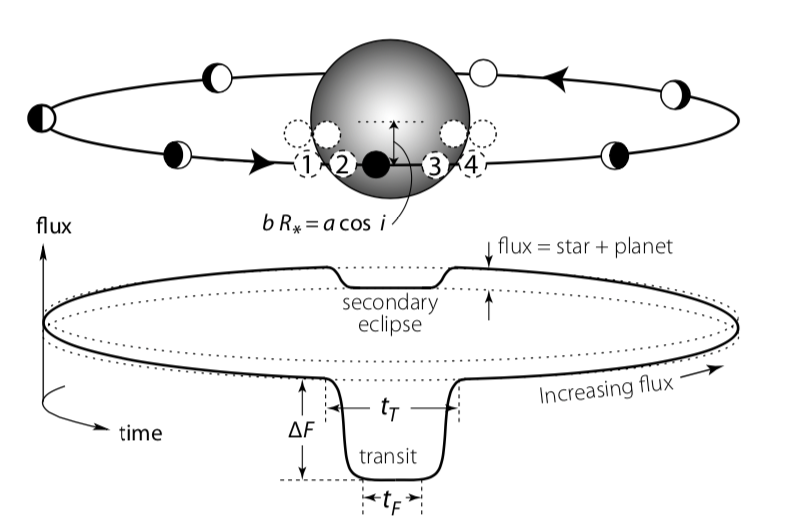
\includegraphics[width=0.8\columnwidth]{imagenes/transit.png}
\caption{Architecture of a transiting exoplanet.}
\label{transit}
\end{figure}

\begin{figure}[H]
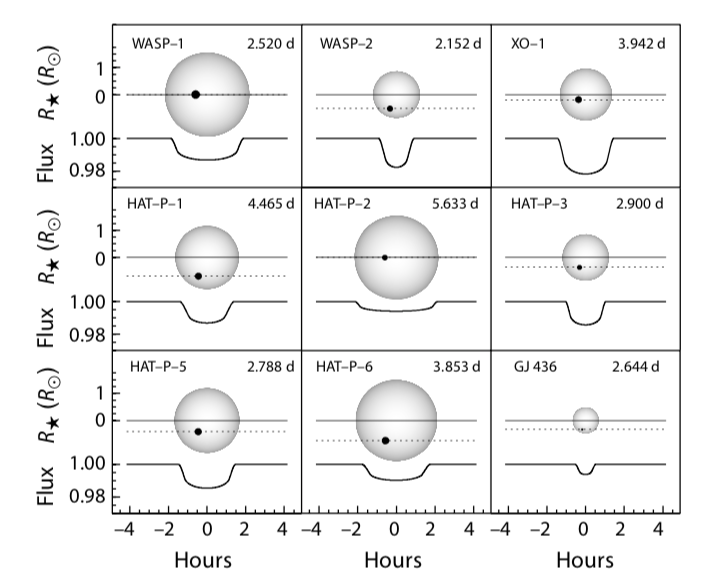
\includegraphics[width=1.0\columnwidth]{imagenes/transit_examples.png}
\caption{Examples of transiting exoplanets and how their light curves differ between them thanks to the physical properties of the exoplanet.}
\label{transit_examples}
\end{figure}



\section{Transit Timing Variations}

\section{The Transit Monitoring in the South project}		% Introduccion
%\input{chap_teoria.tex}		% Marco teórico
%\input{chap_nao_backpack.tex}% Sistema General
%\input{chap_slam_visual.tex}	% Sistema General
%\input{chap_odometria.tex}	% Sistema General
%\input{chap_resultados.tex}	% Resultados
%\input{chap_conclusiones.tex}% Conclusiones

% ----------------------------------------------------------------------
% Glosario
% ----------------------------------------------------------------------
%\input{glosario.tex} % opcional

% ----------------------------------------------------------------------
% Bibliografía
% ----------------------------------------------------------------------

\addcontentsline{toc}{chapter}{Bibliography}
\bibliographystyle{plain}
{\small
\bibliography{bibliografia}
}

% ----------------------------------------------------------------------
% Apéndice
% ----------------------------------------------------------------------

%\begin{appendices}
%\input{apendice_nao_datasheet.tex} 	     % especificaciones del NAO
%\input{apendice_setup_experimental.tex}  % setup experimental
%\input{apendice_lie.tex} 	             % grupos de Lie
%\input{apendice_intentos.tex}	         % Lo que se intentó y no funcionó
%\input{apendice_imu.tex}	             % derivacion de modelo cinemático de la IMU
%\input{apendice_agradecimientos.tex}	 % agradecimientos
%\end{appendices}

\end{document}
\grid
